\section{Requisitos e Arquitetura}
\label{sec:arquitetura}

\subsection{Análise de contexto}

\subsubsection{Visão geral}

    O sistema proposto é um aplicativo para dispositivos móveis que visa facilitar a navegação pelo campus da UFMS, em Campo Grande.  A principal responsabilidade do aplicativo é fornecer informações sobre a localização de prédios, serviços e pontos de interesse no campus, bem como permitir que usuários sugiram adições de novos pontos de interesse e atualizações de informações.

\subsubsection{Condições Restritivas}

    O aplicativo é projetado exclusivamente para dispositivos móveis com sistema operacional Android, tendo o Android 6.0 (API 23) como versão mínima suportada. O aplicativo também exige conexão com a internet para funcionar corretamente.

\subsubsection{Benefícios}

    O aplicativo auxiliará estudantes, professores, visitantes e demais usuários do campus a se localizarem e a encontrarem informações sobre os prédios e serviços disponíveis. Além disso, o aplicativo permitirá que usuários sugiram adições de novos pontos de interesse e atualizações de informações, contribuindo para a melhoria contínua do aplicativo.

\subsection{Analise de requisitos}

\subsubsection{Metodologia}

    Para o desenvolvimento do aplicativo, foi realizado o levantamento de requisitos através de reuniões com a equipe de desenvolvimento. Novos requisitos se mostraram importantes conforme o avanço do desenvolvimento dos requisitos anteriormente propostos.

\subsubsection{Lista de Atores}

    Foram identificados três tipos de atores:

    \begin{itemize}
        \item \textbf{Usuário comum não logado}: Tem acesso aos locais e suas respectivas informações, além dos filtros de buscas. Pode se cadastrar, logar ou recuperar o seu perfil de usuário no sistema.
        \item \textbf{Usuário comum logado}: Tem acesso aos mesmos privilégios do usuário comum não logado, com a adição de: Permissão para alterar informações de seu perfil de usuário, favoritar e avaliar locais, visualizar o registro dos últimos locais acessados, sugerir a adição ou alteração de locais. 
        \item \textbf{Administrador}: Possui permissões de administrador do sistema, pode adicionar ou alterar locais.
    \end{itemize}

\subsubsection{Lista de Funcionalidades}

    As funcionalidades desenvolvidas para a aplicação e os atores responsáveis estão registrados na tabela 1:

    \begin{table}[h]
        \begin{tabularx}{\textwidth}{|X|X|}
            \hline
            \textbf{Funcionalidade} & \textbf{Ator(es)} \\ \hline
            Visualizar informações de locais & Qualquer usuário \\ \hline
            Buscar ou filtrar por locais & Qualquer usuário \\ \hline
            Cadastrar conta & Usuário não logado \\ \hline
            Fazer login & Usuário não logado \\ \hline
            Recuperar conta & Usuário não logado \\ \hline
            Editar perfil de usuário & Usuário comum logado e Administrador \\ \hline
            Favoritar locais & Usuário comum logado e Administrador \\ \hline
            Avaliar locais & Usuário comum logado e Administrador \\ \hline
            Visualizar registros de locais acessados & Usuário comum logado e Administrador \\ \hline
            Sugerir adição ou alteração de locais & Usuário comum logado \\ \hline
            Adicionar ou alterar locais & Administrador \\ \hline
        \end{tabularx}
        \caption{Funcionalidades e Atores do aplicativo Encontre na UFMS}
        \label{tab:funcionalidades-atores}
    \end{table}
    \FloatBarrier
\subsection{Requisitos}
\subsubsection{Diagramas de caso de uso}

    Casos de uso são unidades de interação entre um sistema e um usuário, que podem ser humanos ou máquinas. Eles são utilizados para descrever como o sistema deve se comportar quando estiver pronto, eles não ditam como o sistema deve ser construído mas define os objetivos que a construção deve atingir. Os casos de uso da aplicação foram definidos com base nas funcionalidades propostas, como não há um cliente definido, o comportamento do sistema foi modelado e definido através de reuniões com a equipe de desenvolvimento.

    Diagramas de casos de uso são resumos dos casos de uso que mostram de maneira simplificada todas as interações possíveis do usuário com o sistema. Os diagramas de casos de uso foram divididos em três partes: Usuário não logado, Usuário logado e Administrador. Abaixo estão representados os diagramas de casos de uso para cada um dos atores nas figuras 1, 2 e 3.


    \begin{figure}[h]
        \centering
        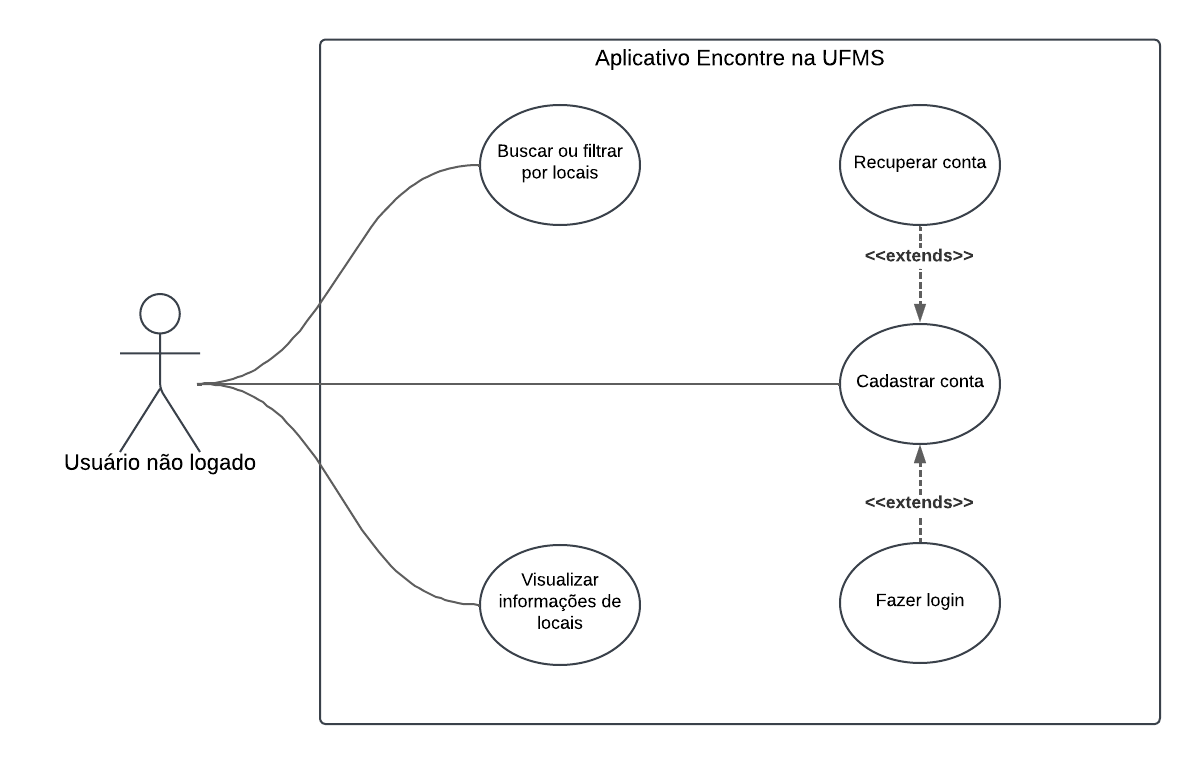
\includegraphics[width=0.7\textwidth]{imagens/usuarioNaoLogado.png}
        \caption{\scriptsize Diagrama de casos de uso (Usuário Não logado)}
        \label{fig:casosDeUsoUsuarioNaoLogado}
    \end{figure}

    \begin{figure}[h]
        \centering
        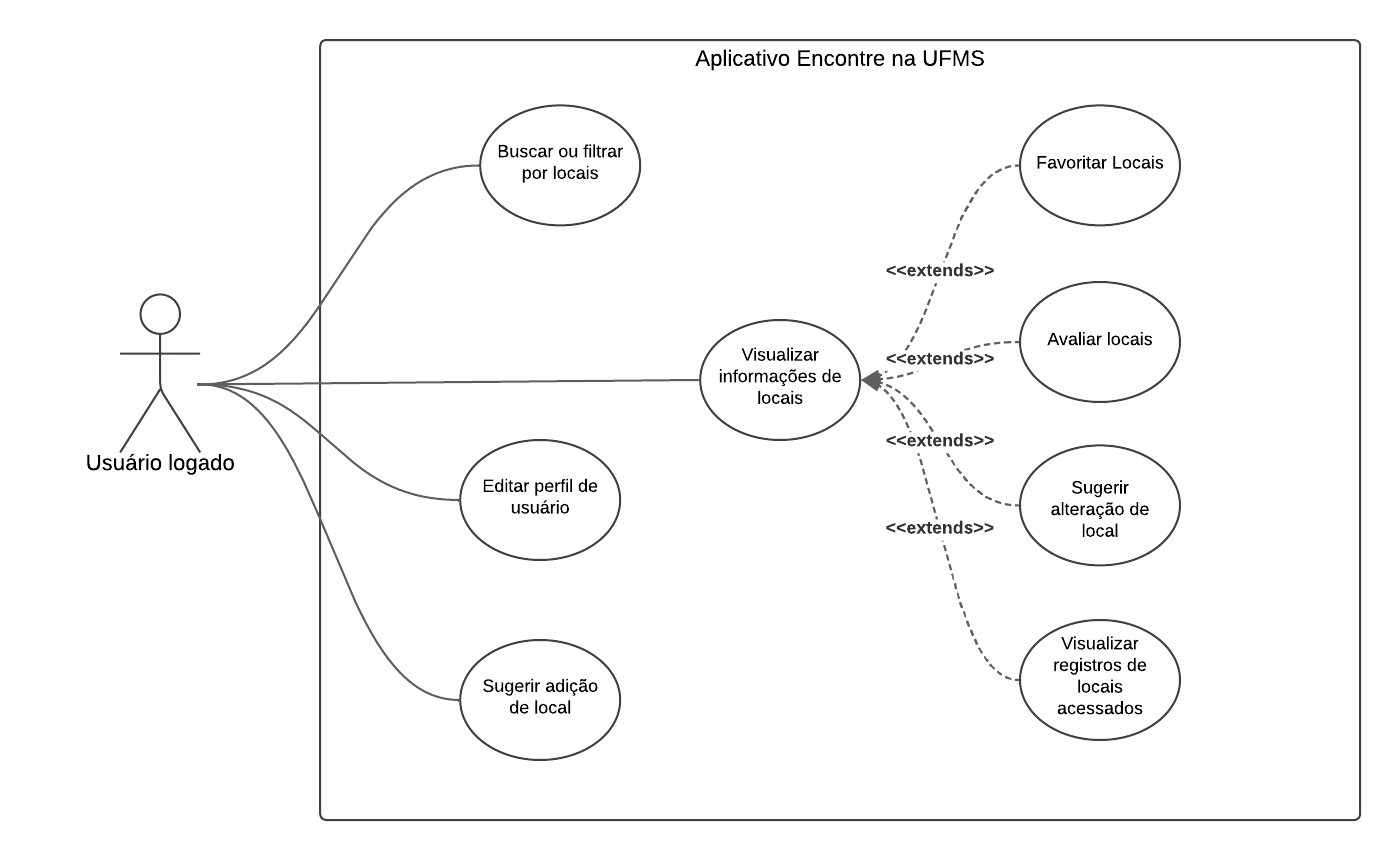
\includegraphics[width=0.7\textwidth]{imagens/usuarioLogado.png}
        \caption{\scriptsize Diagrama de casos de uso (Usuário logado)}
        \label{fig:casosDeUsoUsuarioLogado}
    \end{figure}

    \begin{figure}[h]
        \centering
        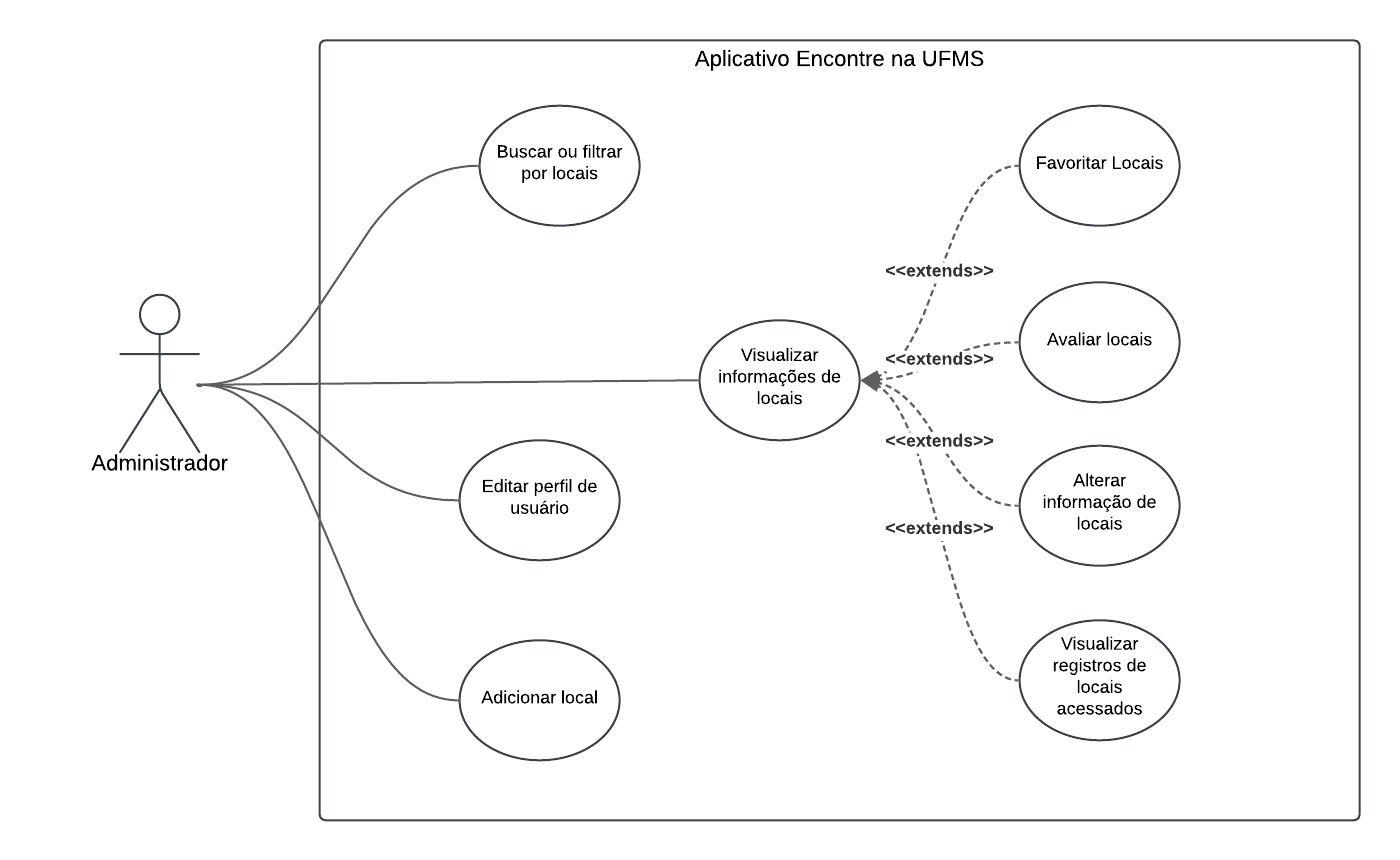
\includegraphics[width=0.7\textwidth]{imagens/administrador.png}
        \caption{\scriptsize Diagrama de casos de uso (Administrador)}
        \label{fig:casosDeUsoAdministrador}
    \end{figure}
    \FloatBarrier

\subsubsection{Especificação dos Requisitos de Software}

    Os requisitos são dividos entre os Requisitos Funcionais e Não-Funcionais. Abaixo, estão listados alguns dos requisitos funcionais descritos no \textit{Documento de Requisitos Aplicativo Encontre na UFMS} \cite{documentoRequisitosAplicativoEncontreNaUFMS}:
    
    \begin{itemize}
      \item \textbf{Listagem de pontos importantes}: O sistema deve listar pontos importantes do campus de Campo Grande da UFMS. Exemplo: Blocos Acadêmicos, Bancos, Pontos Turísticos, Restaurantes, etc.
      \item \textbf{Listagem de informações detalhadas}: O sistema deve fornecer informações detalhadas a respeito de um determinado local, tais como: Nome, endereço, telefone, horário de funcionamento, fotos, entre outras informações.
      \item \textbf{Redirecionamento para o Google Maps}:  O sistema deve oferecer um link que redirecione o usuário para o aplicativo ou página na internet do Google Maps \cite{maps2005} com o endereço do local inserido.
      \item \textbf{Busca de pontos específicos}: O sistema deve permitir que o usuário busque um ponto específico utilizando o nome do local e/ou filtros de busca.
      \item \textbf{Login}: O sistema deve permitir que o usuário faça login, além de possibilitar o cadastro e a recuperação de conta.
      \item \textbf{Favoritar}:  O sistema deve permitir que o usuário favorite os locais de interesse.
      \item \textbf{Avaliar}:  O sistema deve permitir que o usuário avalie os locais, utilizando uma escala de 1 a 5 estrelas.
      \item \textbf{Criar e alterar locais}: O sistema deve permitir que usuários façam sugestões para inclusão ou alteração de locais.
    \end{itemize}
    
    O sistema visa oferecer ao usuário uma experiência de busca e localização eficiente, com uma interface amigável e intuitiva que permite navegar e encontrar informações úteis sobre cada local. Além disso, possui funcionalidades como redirecionamento para o Google Maps \cite{maps2005}, a fim de traçar rotas para que o usuário consiga chegar ao local. Também inclui funcionalidades de cadastro, login e recuperação de conta, permitindo ao usuário usufruir de opções como avaliação de locais, favoritá-los e sugerir novos locais ou editar locais existentes no aplicativo.

\subsubsection{Diagrama de Classes}

    O diagrama de classes apresenta as classes do sistema, seus atributos e suas relações, sendo representado pela Figura 4.

    \begin{figure}[h]
        \centering
        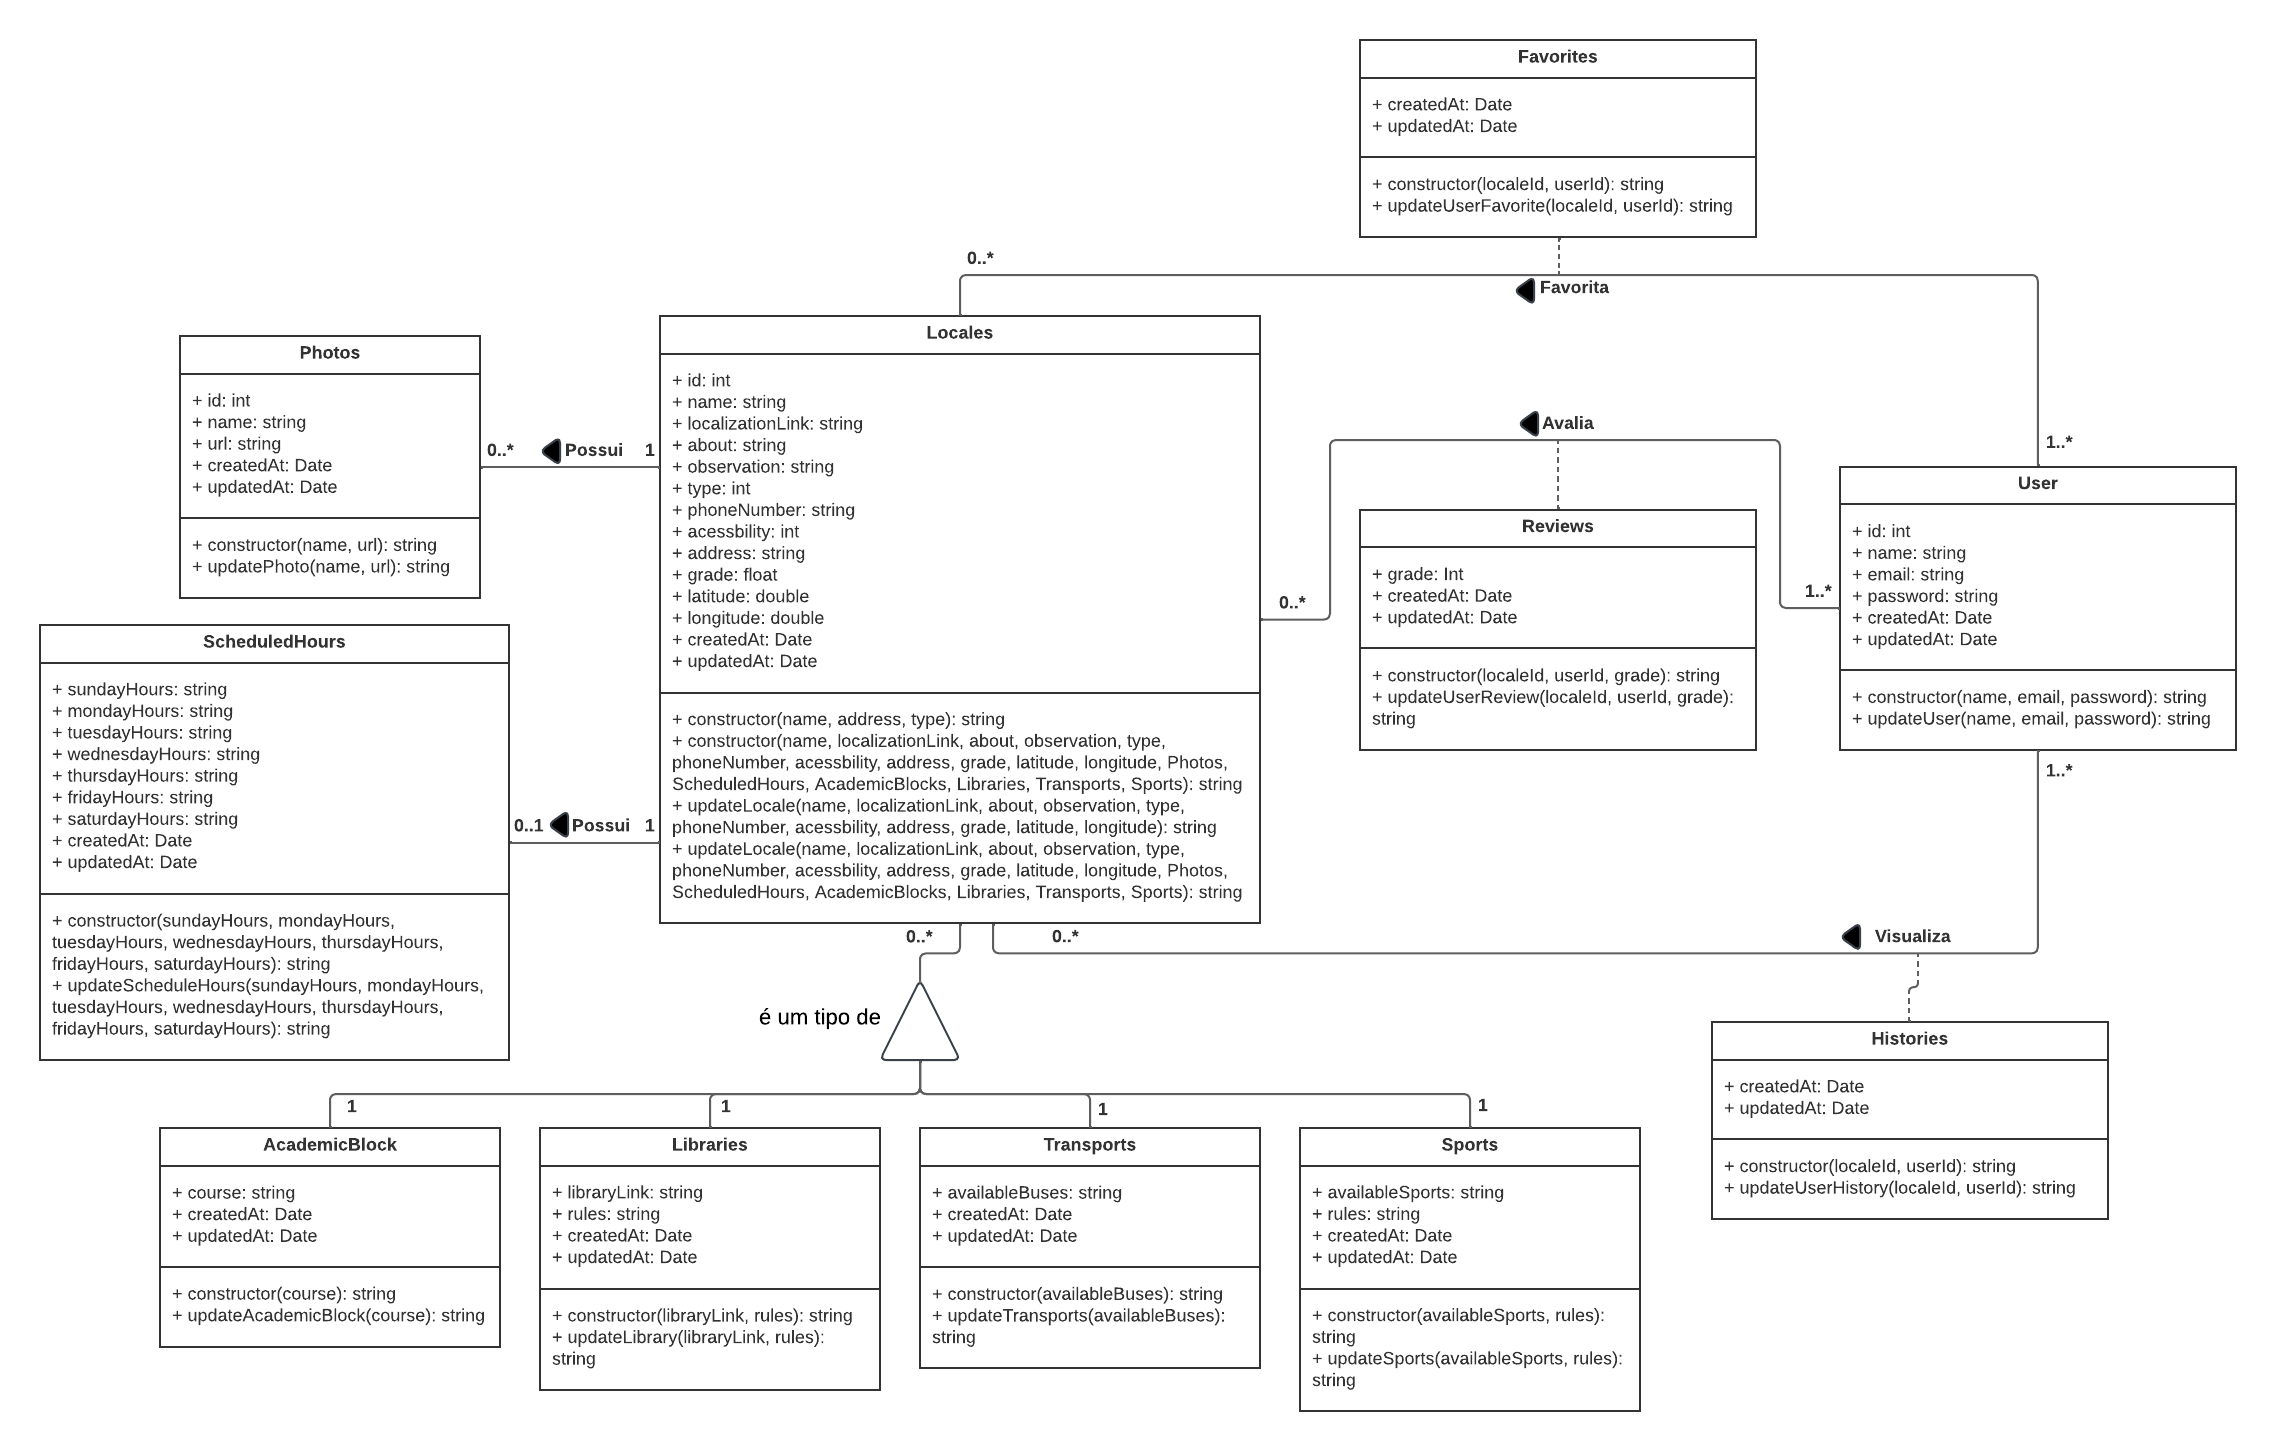
\includegraphics[width=1\textwidth]{imagens/diagramaDeClasses.png}
        \caption{\scriptsize Representação do diagrama de Classes utilizando o LucidCharts \cite{lucidCharts}}
        \label{fig:diagramaDeClasses}
    \end{figure}